Predictions made by statistical models, certain classes of scientific data, and data extracted from disagreeing sources are all instances of data that can be described (i.e., via probability distribution), but not specified exactly.  Measurements have error margins while predictions are typically drawn from well known distributions.  Traditional database management systems (DBMS) are ill-equipped to manage this kind of uncertainty.  For  example, consider  a predictive model  for customer orders based  on trends extrapolated  from historical data.   While a traditional  DBMS can process  queries on  a sampled  order data\-base (one possible  concrete database without  uncertainty in it), if  it is somehow instantiated  from the  model, it is  not equipped  to provide statistical information about quality of the estimates it generates as a result.

Probabilistic  database  management  systems \cite{dalvi07efficient, WidomTrio2008, KochMayBMS2008, SD2007, ORION, MCDB, BayesStore} aim at providing better support for querying uncertain data.  The core problem in query processing in probabilistic databases is computing probabilities of events, moments, and histograms of distributions defined by queries on the uncertain state.  This includes, for example, the computation of expectations of aggregates (e.g., the expected aggregate revenues of a company for the next quarter) and the computation of probabilities of events definable by queries (e.g., the probability that the total sales will exceed a certain amount).

Technically, computing moments in the continuous case calls for the numerical integration of rather complicated functions of the form $E[q] = \int_{\vec x} p(\vec{x}) \cdot q(\vec{x}) \; d\vec{x}.$
%cite Importance Sampling, Montecarlo, Veach, some physics papers?  Look through NR.
This class of integral is one that has been studied extensively; many techniques, both exact and approximate, have been developed to solve it efficiently.  However, these techniques frequently require an intimate knowledge of the integral being computed.  Many are applicable only to specific instances of this problem, while others involve arbitrary manipulations and evaluations of $p(\vec x)$ and $q(\vec x)$.  In short, efficient solutions to general probabilistic queries require the query engine to maintain a comprehensive representation of uncertainty in the data.

This paper presents the PIP, a probabilistic database system for computes statistical measures in a general, algorithm-independent way.  PIP's architecture provides a framework that enables a wide variety of integration techniques within a single probabilistic database engine.  By maintaining lossless representations of uncertainty throughout the query evaluation process, PIP can compute statistical properties using techniques that exploit characteristics of the expression being measured.  Even with relatively straightforward integration techniques and simple queries, this additional knowledge has a profoundly positive effect on the efficiency of the computation and the accuracy of the results.

Accuracy is particularly relevant in cases where the integral has no known closed form and sampling techniques must be used to estimate the integral's value.  This is the case in a surprising range of practical applications, even when strong simplifying assumptions are made about the input data.  For example, even if the input data contains only individual uncertain values that are independent from one another and is sampled from well-studied distributions such as the normal distribution, it is still possible for queries to create complex statistical dependencies in their own right.  It is well known, at least in the discrete case, that related algebra on block-independent-disjoint tables can construct any finite probability distribution\ \cite{1325861,IL1984}.

%

\begin{figure}[!]
\begin{center}
\begin{tabular}{rc}
& Query
\\
%\\
%\hline
\\
\begin{tabular}{r}
query \\
evaluation
\end{tabular}
&
\framebox{
\begin{tabular}{c}
\framebox{
\begin{tabular}{p{4.2cm}}
computing probabilities, \\
moments, and statistical tests
\end{tabular}
}
\\[3ex]
\framebox{
\begin{tabular}{p{4.2cm}}
query plans on c-tables
\end{tabular}
}
\end{tabular}
}
\\[7ex]
\begin{tabular}{l}
data \\
store
\end{tabular}
&
\framebox{
\begin{tabular}{c}
\framebox{
\begin{tabular}{p{4.2cm}}
(probabilistic) c-tables
\end{tabular}
}
\\[2ex]
\framebox{
\begin{tabular}{p{4.2cm}}
succinct representation of \\
joint distribution of random \\
variables (exchangeable)
\end{tabular}
}
\end{tabular}
}
\end{tabular}
\end{center}
\caption{Pip Query Engine Architecture.}
\label{fig:arch}
\end{figure}



\begin{figure}
\begin{center}
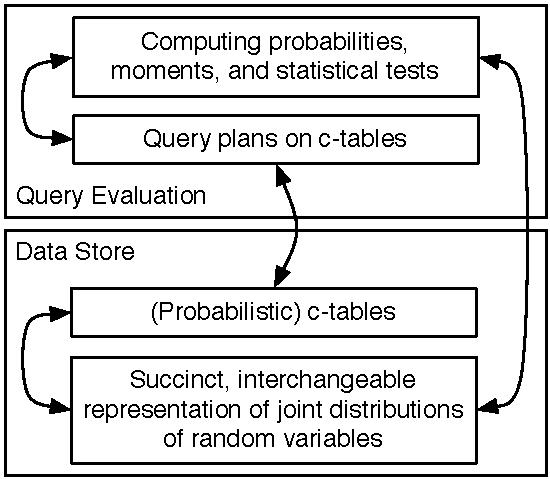
\includegraphics[width=2in]{graphics/arch.pdf}
\caption{Pip Query Engine Architecture}
\label{fig:arch}
\end{center}
\end{figure}

PIP maintains a logical separation between those components of a query that manipulate uncertain data symbolically, and those components that generate statistical measures and graphical representations of the data.  This separation is shown in Figure \ref{fig:arch}.  The data management and storage layers are aware of random variables in the data and are able to manipulate that data symbolically, but treat the component variables as opaque.  This opaqueness allows PIP to be easily extended for use with arbitrary distributions, and allows these distributions to interact with each other naturally.  When it becomes necessary to compute concrete values like expectations, the final layer is presented with a complete encoding of the uncertainty in the query results.  

Superficially similar to so called {\em VG Functions} as seen in \cite{MCDB}, PIP garners even more benefit by allowing developers to specify supplemental information (eg, the PDF and CDF) about distributions they integrate into PIP.  Because PIP's symbolic encoding of random values contains references to the distribution each variable is chosen from, PIP can make use of this information.  For example, the probability of a variable falling within specified bounds can be computed with two evaluations of the variable's cumulative distribution function.  This pass-through approach to query evaluation makes it possible for PIP to support a wide range of integration techniques.

Last but not least, PIP's lossless symbolic representation facilitates saving intermediate query state (ie, materializing views).  Subsequent statistical measurements made on queries over materialized views will not be biased by estimation errors made during the creation of these views.  This is especially useful when a significant fraction of query processing time is devoted to managing deterministic data (eg, to obtain distribution parameters).  Not only can this accelerate processing of commonly used query segments, but it makes online sampling feasible; the sampler need not evaluate the entire query from scratch to generate additional samples.

{\em Monte Carlo integration}\/.
There is one conceptually simple technique, however, that  allows for the (approximate) numerical integration of even  the most general  functions, including those occurring in  probabilistic data  processing: Monte Carlo integration \cite{montecarlo}. Conceptually, to compute an expectation, one simply approximates   the  integral  by  taking $n$ samples $\vec{x}_1, \dots, \vec{x}_n$ for $\vec{X}$ from $p$  and  taking  the  average of the $q$ values,
%
\begin{equation}\label{eq:mc_expectation}
\frac{1}{n} \cdot \sum_{i=1}^n q(\vec{x}_i).
\end{equation}

In general, even taking a sample from a complicated PDF is difficult.  Constraints imposed by queries break assumptions of normalization on $p(\vec x)$ and require that the sampling technique account for them or lose precision.  A variety of techniques exist to address this problem, from straightforward rejection sampling, where constraint-violating samples are repeatedly discarded, to more heavy duty Markov-chain Monte Carlo (MCMC, cf.\ e.g., \cite{GRS1995}) style techniques such as the Metropolis-Hastings algorithm\cite{metropolis,GRS1995}. 

MCMC is used pervasively in science, for instance in simulating  physical processes  or reconstructing  genomes  from short sequence data.  It is also extensively used in a new generation of Artificial Intelligence probabilistic inference systems whose aims are somewhat related to those of probabilistic database systems \cite{RD2006, BLOG}.

{\em Challenges  of sampling-based query processing}\/.  To  summarize, a Monte Carlo simulation/sampling-based approach is  a  natural  design  choice  for  probabilistic  database  systems. However,  a  Monte Carlo  approach  leaves  us  with the  problems  of efficiently creating samples (the  techniques we have discussed so far call for samples that are  entire databases, not just atomic values or tuples) and computing sufficiently  many samples to yield satisfactory results.  Additionally, we would like to know how many samples we need to get certain error bounds.


Recently,  the paper  \cite{MCDB} on  the MCDB  system  has promoted an integrated  sampling-based  approach to  probabilistic databases.  Conceptually,  MCDB uses a {\em sample-first}\/ approach: it   first  computes  samples  of  entire databases and then processes queries  on these samples.  This is a very general and flexible approach, largely due to its modular approach to probability distributions via black box sample generators called VG Functions.  However, in its basic form, parallel evaluation over many sampled databases is very inefficient; as an optimization, samples are computed lazily and bundled by tuple.  

{\em  Conditional tables}\/  (c-tables, \cite{IL1984})  are relational tables in which tuples have associated conditions expressed as boolean expressions over  comparisons of random variables  and constants. C-tables are a natural way to  represent  the  {\em  deterministic skeleton}\/  of a probabilistic relational  database in  a succinct  and tabular  form.  That  is, complete information  about uncertain data is encoded using random  variables, excluding only  specifications  of the  joint  probability  distribution of  the random  variables   themselves.   This  model   allows  representation of  input databases  with  nontrivial statistical  dependencies that are normally associated with graphical models. 

For discrete probabilistic  databases, a canon of systems has been developed that essentially uses  c-tables, without referring to them as such. MystiQ  \cite{dalvi07efficient}  uses  c-tables internally  for  query processing  but  uses  a  simpler  model for  input  databases.   Trio \cite{WidomTrio2008}  uses  c-tables with  additional  syntactic sugar  and calls conditions {\em lineage}\/.  MayBMS \cite{AJKO2008}  uses a  form of  c-tables called  U-relations that define how relational algebra representations of queries can encode the corresponding condition transformations.


Using c-tables  for  query evaluation  allows  compositional  transformation of probabilistic  database representations, thus allowing a single c-table to sumultaneously represent  all possible worlds  (sample databases) at once. Samples can then be drawn as late in the query evaluation process as possible,  after all relational algebra work is finished. This has  many advantages over  sample-first approaches.
\begin{itemize}
\addtolength{\topsep}{-0.3ex}
\addtolength{\labelsep}{-0.3ex}
\addtolength{\itemsep}{-1ex}
\item
Evaluating relational algebra on c-tables is  essentially as efficient as processing  the same algebra queries on a  single  MCDB  sample. By evaluating query operations on  the c-table, we may be able  to filter out tuples that would otherwise have to be  sampled before being dropped  in a sample-first approach.  This allows us  to sample more selectively  for the needs of  the query and produce higher-quality results with  the same amount of work as in a sample-first approach. This  is particularly important for highly  selective queries or aggregation queries with group-by constructs, for which relatively low numbers   of   samples   (as   MCDB   produces   them) result in notoriously imprecise answers.

\item
Computing further samples in the c-tables approach is  cheaper than in  MCDB, because  we do  so only  after most  of the querying  work  has been  done.   Thus,  using  c-tables, multiple sample sets may be produced without incurring query processing overheads more than once.  This is particularly important in online  sampling, where we want to  quickly produce  a first  result based on few samples and then  improve on the result by computing more samples until the user is satisfied with the result.

\end{itemize}


\begin{example}\em
\label{ex:intro}
Suppose a database captures customer orders expected for the next quarter,
including prices and
and destinations of shipment. The order prices are 
uncertain, but a probability distribution is assumed.
The database also stores
distributions of shipping durations for each location.
Here are two c-tables defining such a probabilistic database:
\[
\begin{tabular}{c|ccc}
Order & Cust & ShipTo & Price \\
\hline
& Joe & NY & $X_1$ \\
& Bob & LA & $X_3$ \\
\end{tabular}
%\hspace{5mm}
\]\[
\begin{tabular}{c|cc}
Shipping & Dest & Duration \\
\hline
& NY & $X_2$ \\
& LA & $X_4$ \\
\end{tabular}
\]
We assume a suitable specification of the joint distribution $p$ of the random
variables $X_1,\dots,X_4$ occurring in this database.

Now consider the query
\begin{verbatim}
select expected_sum(O.Price)
from   Order O, Shipping S
where  O.ShipTo = S.Dest
and    O.Cust = 'Joe'
and    S.Duration >= 7;
\end{verbatim}
asking for the expected loss due to late deliveries to customers named Joe,
where the product is free if not delivered within seven days.
%
This can be approximated by drawing a number of samples from $p$
and using formula~\ref{eq:mc_expectation}
to approximate $E[q]$,
where $q$ represents the result of the sum aggregate query on a sample,
here
\[
q(\vec{x}) =
\left\{
\begin{array}{lll}
x_1 & \dots & x_2 \ge 7 \\
0 & \dots & \mbox{otherwise.}
\end{array}
\right.
\]

In a naive sample-first approach, 
if $x_2 \ge 7$ is a relatively rare event, a large number of samples will be
required to compute a good approximation to the expectation.
Moreover, samples also require an effort for customer Bob,
which does not contribute to the result.

Now consider using c-tables. The result of the relational algebra part of the
above query can be easily computed without looking at $f$ as
\[
\begin{tabular}{c|c|c}
R & Price & Condition \\
\hline
& $X_1$ & $X_2 \ge 7$ \\
\end{tabular}
\]
This c-table compactly represents all relevant data still relevant after the
application of the relational algebra part of the query, other than $p$,
which remains unchanged.
Sampling from R to compute
\begin{verbatim}
select expected_sum(Price) from R;
\end{verbatim}
is a much more focused effort.
First, we only have to consider the random variables relating to Joe;
but determining that random variable $X_2$ is relevant while $X_4$
is not requires
executing a query involving a join. We want to do this query first, before
we start sampling.

Second, assume that delivery times are
independent from sales volumes. Then we can approximate the
query result
by first sampling an $X_2$ value and only sampling an $X_1$ value if $X_2 \ge 7$.
Otherwise, we use $0$ as the $X_1$ value.
If $X_2 \ge 7$ is relatively rare (e.g., the average shipping times to NY are
very slow, with a low variance), this may reduce the amount of samples
for $X_1$ that are first computed and then discarded without seeing use
considerably.
If CDFs are available, we can of course do even better.

In Section \ref{sec:evaluation} we compare the c-tables approach to a very basic, 
naive sample-first approach.  Note however, that \cite{MCDB} describes a number of 
optimizations that MCDB uses to obtain some of the advantages gained by using c-tables.
%
\punto
\end{example}


The  c-tables  approach has  never  been used  to build  a
probabilistic  database  management  system that  supports  continuous
probability  distributions.
%
ORION \cite{ORION} is a probabilistic database management system for
continuous distributions that can alternate between sampling
and transforming distributions. However, their representation
system is not based on c-tables but essentially on the
world-set decompositions of \cite{AKO07WSD}, a factorization
based approach related to graphical models.
Selection queries in this model may require an exponential blow-up in the
representation size, while selections are efficient in c-tables.


{\em PIP}\/'s approach encompasses and extends both the strengths of discrete systems that use c-tables such as MystiQ and MayBMS, as well as the generality of MCDB's Monte-Carlo approach.  It supports both discrete and continuous probability distributions, powerful correlations definable by queries, expectations of aggregates and distinct-aggregates with or without  group-by,  and the computation of confidences. The detailed technical contributions of this paper are as follows.


\begin{itemize}
\addtolength{\topsep}{-0.3ex}
\addtolength{\labelsep}{-0.3ex}
\addtolength{\itemsep}{-1ex}
\item
We study query evaluation using probabilistic conditional tables, for
relational algebra, aggregates, and the computation of expectations and
probabilities.

\item
We present the architectural and language design decisions made in the
PIP system, and show how the various techniques introduced combine into
a unified whole.

\item
We provide experimental evidence for the competitiveness of our approach, comparing PIP with a reimplementation of the refined sample-first approach taken by MCDB.  We use a common codebase for both systems based on Postgres to enable fair comparison. We show that PIP is in general competitive to MCDB (it essentially never does more work) and can reduce the amount of work needed to compute the same number of samples substantially; in other cases, delaying sampling using c-tables to a stage where more is known about what samples are needed; This added information can lead to the same number of samples giving better quality results in PIP than in MCDB.
\end{itemize}

The structure of this paper is as follows. Section~\ref{sec:background} presents probabilistic c-tables, our database model, and the conceptual  evaluation of queries on probabilistic c-tables. Section~\ref{sec:sampling} studies sampling, Monte
Carlo integration, and other mechanisms for computing integrals.  In Section~\ref{sec:design}, we present a high level view of PIP in the abstract.   Section~\ref{sec:implementation} discusses details of the implementation of PIP and our reimplementation of MCDB.  Finally, in Section~\ref{sec:evaluation}, we present the outcomes of our experiments with PIP and our MCDB reimplementation.